\documentclass[a4paper,12pt]{article}
\usepackage{graphicx}
\usepackage{amsmath, amssymb}
\usepackage{hyperref}
\usepackage{tikz}
\usepackage[backend=biber, style=numeric, citestyle=ieee]{biblatex}

\addbibresource{references.bib}


\title{Newton's Law of Acceleration: Technical Paper for Activity 1}
\author{Janelle Lastimado \\
John Paul Memoracion \\ 
Nikki Shane Mercado \\
Gian Myrl Renomeron}
\date{January 28, 2025}

\begin{document}

\maketitle

\begin{abstract}
    Newton's Second Law of Motion states that the acceleration of an object depends upon the force applied to it and its mass. This study aims to find how acceleration varies in two conditions: (1) when force varies while mass remains constant, and (2) when mass varies while force remains constant. A rolling cart was used to keep friction to an absolute minimum to take measurements in both scenarios. By measuring acceleration both experimentally and theoretically, this comparison of theory to experiment gave way to proof that indeed mass can be neglected as force is increased while vice versa is expected. Experimental vs theoretical values vary marginally, mainly because of the existence of friction and the likely occurrence of the experimental error due to measurement uncertainty. Overall, the results agree with Newton's Second Law, and therefore it has practical applicability.
\end{abstract}

\section{Introduction}
Newton's Second Law of Motion states the basic relationship between force, mass, and acceleration. As expressed mathematically in the formula F = ma, an object's acceleration varies inversely with its mass and directly with the net force acting on it \cite{halliday2021fundamentals}. It has many applications in physics, engineering, and other scientific domains and is key to understanding motion. \\

Based also on this, the scientists were able to conclude that the external forces occurring on an object are responsible for its movement. The acceleration that results from applying a force is dependent on the mass of the object. While a larger, massive object needs more effort to attain the same acceleration, a bigger force results in a higher acceleration \cite{knight2017physics}. \\

In experimental physics, one is obliged to grasp the relationship between force, mass, and acceleration to develop an accurate motion model. In this kind of experiment, scientists often use pulleys or rolling carts on frictionless tracks to study these relationships and to find out results, as it is more accurate when there is less friction, which one can understand better the concept of Newton's second law because it ensures that external forces do not change the results in a significant way \cite{young2020university}. \\

Therefore, this experiment uses a rolling cart system to explore the relationship between force, mass, and acceleration. It was to see how acceleration changes when force changes while mass stays constant and how it reacts when mass changes while force stays constant. The results of this experiment are not only important information about Newton's law of acceleration but also provide a crucial understanding of its real-world applicability.

\section{Materials and Methodology}

\begin{figure}[h]
    \centering
    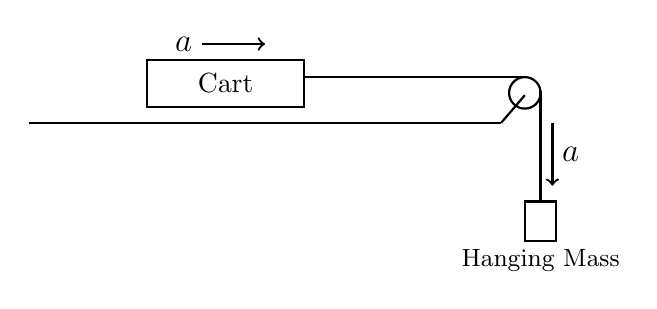
\begin{tikzpicture}
        % Draw the surface
        \draw[thick] (-3,0) -- (3,0); % Table/Track

        % Draw the cart
        \draw[thick] (-1.5,0.2) rectangle (0.5,0.8); % Cart body
        \node at (-0.5, 0.5) {Cart};

        % Draw the pulley
        \draw[thick] (3.3, 0.38) circle (0.2); % Pulley wheel
        \draw[thick] (3,0) -- (3.3,0.35); % Pulley arm

        % Draw the string
        \draw[thick] (0.5, 0.58) -- (3.3, 0.58); % Horizontal part
        \draw[thick] (3.5, 0.4) -- (3.5, -1); % Vertical part

        % Draw the hanging mass
        \draw[thick] (3.3,-1) rectangle (3.7,-1.5); % Hanging mass
        \node at (3.5,-1.75) {\small Hanging Mass};

        % Draw acceleration vector
        \draw[->, thick] (-0.8, 1) -- (0, 1);
        \node[left] at (-0.8, 1) {\large $a$};

        % Draw acceleration vector for the hanging mass
        \draw[->, thick] (3.65,0) -- (3.65,-0.8);
        \node[right] at (3.65,-0.4) {\large $a$};

    \end{tikzpicture}
    \caption{Experimental setup}
    \label{fig:cart_pulley}
\end{figure}

\subsection{Materials}
Below are the list of materials used in the experiment
\begin{itemize}
    \item Rolling cart
    \item String
    \item Weight hanger
    \item Slotted mass
    \item Pullery
    \item Meterstick
    \item Stopwatch
\end{itemize}

\subsection{Methodology}
Two types of experiments was done, one where \textit{mass is constant and the force varies} and one where the \textit{force is constant and the mass varies}. The goal of this experiment is

\begin{enumerate}
    \item To determine the relationship between acceleration and force when the mass is kept constant, and
    \item To determine the relationship between acceleration and mass when the force is kept constant
\end{enumerate}

\subsubsection{Procedures}

\paragraph{Experiment 1: Mass constant, Force varies}
\begin{enumerate}
    \item Weigh the cart. Set up the apparatus as shown in the diagram (see Figure \ref{fig:cart_pulley})
    \item Add enough small masses to the wight hanger so that the cart will move uniformly when it is given a slight push. This serves as counterweight. This should stay in the weight hanger throughout the experiment but should not be considered as a force.
    \item Place 50 g on the weighthanger. This serves as the first force. Mark the initial position of the cart. Measure the time it takes for the cart to travel a certain distance.
    \item Run two more trials by increasing the force. Fro every change in force, measure the time it takes for the cart to travel the distance as in step 3.
\end{enumerate}

\paragraph{Experiment 2: Force constant, Mass varies}
\begin{enumerate}
    \item Remove the other masses on the weight hanger leaving only 150g which serves as the constant force. Retain also the counterweight. Load the cart with 300g. Measure the time required for the cart to travel the same distance.
    \item Run two more trials by decreasing the mass of the system. Remove 100g mass from the cart, then 200g more mass. For every change in mass, measure the time needed to travel the same distance.
\end{enumerate}

\paragraph{Computation and Analysis}
\begin{enumerate}
    \item Calculate the acceleration (theoretical values) corresponding to different focuses using Newton's law of acceleration, \( F = ma \) and the experimental values using the linear motion equation
\end{enumerate}



\section{Results and Discussion}
Below is the data and result of the experiments.

\subsection{Experiment 1: Mass constant, Force varies}
\begin{table}[h]
    \centering
    \renewcommand{\arraystretch}{1.2}
    \makebox[\textwidth]{ 
    \begin{tabular}{|c|c|c|c|c|c|c|}
        \hline
        \textbf{Trial} & \textbf{Mass (kg)} & \textbf{Force (N)} & \textbf{Time (s)} & \textbf{Distance (m)} & \multicolumn{2}{c|}{\textbf{Acceleration (m/s\(^2\))}} \\
        \cline{6-7}
        & & & & & \textbf{TV} & \textbf{EV} \\
        \hline
        1 & 0.033 kg & 0.49 N & 0.32 s & 0.71 m & 14.8 m/s\(^2\) & 13.87 m/s\(^2\) \\
        2 & 0.033 kg & 0.539 N & 0.29 s & 0.71 m & 16.3 m/s\(^2\) & 16.88 m/s\(^2\) \\
        3 & 0.033 kg & 0.588 N & 0.27 s & 0.71 m & 17.8 m/s\(^2\) & 19.47 m/s\(^2\) \\
        \hline
    \end{tabular}
    }
    \caption{Results for Experiment 1: Mass constant, Force varies}
    \label{table:exp1}
\end{table}

As one can see in table \ref{table:exp1} for the first experiment, constant mass of cart with varying forces were applied on the cart and their acceleration in theory and actual measurement are very clear. From these values acceleration due to increased force is obtained and it does agree with the second law formulated by Newtons as \( F = ma \), with a constant value of mass in that case it will be more or less proportionate to an acceleration. \\

Experimental acceleration values are quite close to the theoretical one, despite some slight differences. These can be caused by the friction from the surface and air friction around the test body, errors in measurement or reaction time to start and stop the stopwatch. Despite such minute differences, the trend clearly shows that acceleration increases with force, as expected by the theory.

\subsection{Experiment 2: Force constant, Mass varies}
\begin{table}[h]
    \centering
    \renewcommand{\arraystretch}{1.2}
    \makebox[\textwidth]{
    \begin{tabular}{|c|c|c|c|c|c|c|}
        \hline
        \textbf{Trial} & \textbf{Mass (kg)} & \textbf{Force (N)} & \textbf{Time (s)} & \textbf{Distance (m)} & \multicolumn{2}{c|}{\textbf{Acceleration (m/s\(^2\))}} \\
        \cline{6-7}
        & & & & & \textbf{TV} & \textbf{EV} \\
        \hline
        4 & 0.292 kg & 0.49 N & 0.9 s & 0.71 m & 1.68 m/s\(^2\) & 1.75 m/s\(^2\) \\
        5 & 0.242 kg & 0.49 N & 0.8 s & 0.71 m & 2.02 m/s\(^2\) & 2.22 m/s\(^2\) \\
        6 & 0.192 kg & 0.49 N & 0.75 s & 0.71 m & 2.55 m/s\(^2\) & 2.52 m/s\(^2\) \\
        \hline
    \end{tabular}
    }
    \caption{Results for Experiment 2: Force constant, Mass varies}
    \label{table:exp2}
\end{table}


Table \ref{table:exp2} shows the second experiment with constant applied force and varying masses. The trend of the graph shows that with decreasing mass, acceleration increases, which is opposite to what has been observed thus far. The result is, however, perfectly consistent with Newton's Second Law because acceleration depends inversely upon mass when the force is constant \( a = F/m \). \\

Comparing the theoretical (TV) and experimental acceleration values, we can see that they each exhibit the same pattern but with minor differences. The possible reasons for the discrepancies involve inconsistent friction, slight differences in mass distribution, human error in measurement of timing, and variation in force application. Yet despite all of these, the general results point out the expected inverse proportionality between acceleration and mass.

\section{Conclusion}

The experiment was successful in testing the Newton's Second Law of Motion. The investigation found that constant mass allows an increase in force resulting in increased acceleration. An increase in mass with constant force leads to reduced acceleration. Following the expected trends as determined by the equation: \( F = ma \), which also corresponds directly to the relationships between force, mass, and acceleration.

\printbibliography

\end{document}
